\documentclass[a4paper,11pt,oneside]{scrartcl}
\usepackage[utf8]{inputenc}
\usepackage[T1]{fontenc}
\usepackage{lmodern}
\KOMAoptions{DIV=14}
\usepackage[english]{babel}
%
\usepackage{graphicx}
\usepackage{caption}
\usepackage[caption=false]{subfig}
%
\usepackage{chngcntr}
\counterwithout{figure}{section}
\counterwithout{table}{section}
%
\usepackage{xcolor}
\usepackage{url}
%
\usepackage{amsmath,amssymb}
\usepackage{trfsigns}
\usepackage{nicefrac}
\usepackage{comment}
%
\usepackage{tikz}
\usetikzlibrary{shapes.misc}
\tikzset{cross/.style={cross out, draw,
         minimum size=2*(#1-\pgflinewidth),
         inner sep=0pt, outer sep=0pt}}
%
\newcommand{\eq}[1]{Eq. (\ref{#1})}
%
\newcommand{\fscom}[2][red]{\textcolor{#1}{#2}}
\definecolor{CalcColor}{rgb}{0.0,0.0,0.5}
\newcommand{\ExCalcCol}[2][CalcColor]{\textcolor{#1}{#2}}
%\excludecomment{calc}
\includecomment{calc}
%
\title{Frequency response of a 2nd order ordinary differential equation (ODE)
with constant coefficients}
\author{Frank Schultz, fs446}
%
\begin{document}
%
\noindent Uni Rostock, IEF, INT, Signal- \& Systemtheorie, \#24015, SS2019,
\today, CC BY 4.0

\noindent Prof. Sascha Spors, Frank Schultz

\noindent \textbf{Frequency Response of 2nd Order Ordinary Differential Equation (ODE) with
Constant Coefficients given as Laplace Transform}

%##############################################################################
%##############################################################################
\section{Problem Statement / Task}

For the Laplace transform
\begin{align}
\label{eq:H_ODE}
H(s) = \frac{1}{\frac{16}{25} s^2 + \frac{24}{25} s + 1},
\end{align}
here interpreted as an LTI system's transfer function, the frequency response
shall be discussed in terms of the Bode plot.
%
We assume a causal system, thus the region of convergence (ROC) is right of the
right-most pole in the left $s$-plane.
%
Note: The frequency response exists only if the $\Im(s)$-axis is included
in the ROC.

The solution is shown in Fig. \ref{fig:bode_ode}.

\section{Helping Variables and Preliminaries}
It is meaningful to check $H(s)$ against the general forms
\begin{align}
\label{eq:Hs_general}
H(s) = \frac{K}{\frac{1}{\omega_0^2} s^2 + \frac{2 D}{\omega_0} s + 1}
= \frac{K}{\tau_0^2 s^2 + 2 D \tau_0 s + 1},
\end{align}
where $0\leq D \leq 1$ realizes differently damped, stable LTI systems for a
chosen cut frequency $\omega_0=\nicefrac{1}{\tau_0}$.
%
For $D=0$ the poles are located on $\Im(s)$-axis (i.e. semi-stable),
the system behaves very resonant at $\omega_0$.
For higher $D$ this resonant characteristics becomes increasingly
damped, since the poles increasingly move away from the $\Im(s)$-axis.
%
Thus, $D$ is typically termed damping factor.
%
From given $H(s)$ we can state the quantities
\begin{equation}
K=1, \qquad \omega_0^2 = \frac{25}{16} \cdot \frac{1}{\text{s}^2}
\rightarrow \omega_0 = \frac{5}{4} \cdot \frac{\text{1}}{\text{s}},
\qquad D = \frac{3}{5}.
\end{equation}
%
From Fig. \ref{fig:sketch_lambda_plane} we can deduce further helpful variables
(assuming $\sigma_0\geq 0$, $\omega_D\geq 0$, $\omega_0\geq 0$)
\begin{equation}
D = \cos \alpha = \frac{\sigma_0}{\omega_0},\qquad
\omega_D^2 = \omega_0^2 (1-D^2) \quad \rightarrow \quad \omega_D = \omega_0
\sqrt{1-D^2}.
\end{equation}
%
\begin{figure}[b!]
\centering
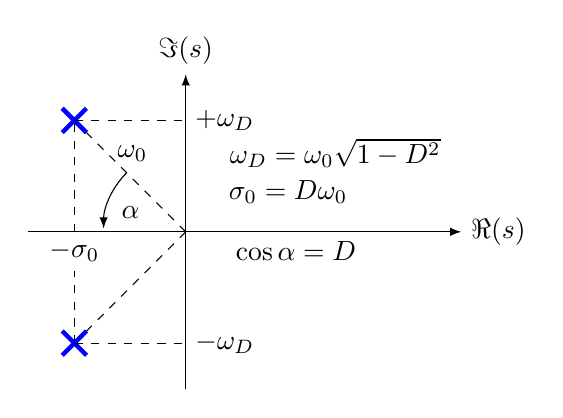
\begin{tikzpicture}
\draw [-latex] (-2,0) -- (3.5,0) node [right]  {$\Re(s)$};
\draw [-latex] (0,-2) -- (0,2) node [above] {$\Im(s)$};
\draw[dashed] (0,0) -- node[pos=0.7, right] {$\omega_0$}(135:2) node[solid, fill=white, cross=6pt, draw=blue, ultra thick] {};
\draw[dashed] (0,0) -- node[pos=0.6, above right] {$ $}(-135:2) node[solid, fill=white, cross=6pt, draw=blue, ultra thick] {};
\draw[dashed] (-1.4142,0) -- (-1.4142,+1.4142);
\draw[dashed] (-1.4142,-1.4142) -- (-1.4142,-0.5) node [left, above] {$-\sigma_0$};
\draw[dashed] (-1.4142,+1.4142) -- (0,+1.4142) node [right] {$+\omega_D$};
\draw[dashed] (-1.4142,-1.4142) -- (0,-1.4142) node [right] {$-\omega_D$};
\draw[black, -latex] (-0.75,0.75) arc (135:180:1);
\node at (1.9,1) {$\omega_D = \omega_0 \sqrt{1-D^2}$};
\node at (1.3,0.5) {$\sigma_0 = D \omega_0$};
\node at (-0.7,0.25) {$\alpha$};
\node at (1.4,-0.25) {$\cos \alpha = D$};
\end{tikzpicture}
\caption{Pole-zero map of 2nd order LTI system under discussion with a complex
conjugate pole pair.}
\label{fig:sketch_lambda_plane}
\end{figure}
%
The two poles of the LTI system under discussion are located at
$s_{\infty,1,2} = -\sigma_0 \pm \im\,\omega_D$.
The quantities are
\begin{equation}
\sigma_0 = \frac{3}{4}\cdot \frac{\text{1}}{\text{s}},\qquad
\omega_D = 1 \cdot \frac{\text{1}}{\text{s}},
\end{equation}
%
and thus $s_{\infty,1,2} = -\frac{3}{4} \pm \im$
omitting the physical unit \textit{second} in the following.
%
Note that the distance $|s_{\infty,1,2}| = \omega_0$.
%
The ROC is $\Re\{s\}>-\frac{3}{4}$ and thus includes the $\Im(s)$-axis.

Note, that in \eq{eq:Hs_general} the first version using $\omega_0$ is
common in filter design, whereas the second version with the time
constant $\tau_0$ is often used in controlling engineering. This is
meaningful since in filter design often the frequency response is to be optimised,
whereas a controller is rather optimised for a dedicated temporal behaviour.
%
The system under discussion is called either a lowpass of 2nd order
(frequency design view) or a PT$_2$-element (controller view).
At the end, this is just naming. More important is that we figure out how to describe its behaviour in the frequency domain in the following. A valuable reference for further reading on he topic is Chapter 6.5.2
in Oppenheim, Willsky, Nawab (1997): "\textit{Signals \& Systems}", Prentice Hall, Upper Saddle River NJ (USA), 2nd edition.




\section{Preparing for Bode Plot}
\subsection{Rational Function in Zero/Pole Notation}
We often discuss LTI systems that are described by a rational function
\begin{align}
\label{eq:Hs_b_a}
H(s) = \frac
{b_M s^M + b_{M-1} s^{M-1} + \dots + b_2 s^2 + b_1 s^1 + b_0 s^0}
{a_N s^N + a_{N-1} s^{N-1} + \dots + a_2 s^2 + a_1 s^1 + a_0 s^0}
\end{align}
with coefficients $b,a \in \mathbb{R}$ and $M,N \in \mathbb{N}$ being the
polynomial orders of numerator and denominator, respectively.
%
Therefore, for \eq{eq:Hs_general} we have $b_0 = K$.
%Using $b$ and $a$
%in such way is a very often used convention.
%

One needs to arrange the vectors / arrays
\begin{align}
b = (b_M, b_{M-1}, \dots, b_2, b_1, b_0)^\mathrm{T}, \qquad
a = (a_N, a_{N-1}, \dots, a_2, a_1, a_0)^\mathrm{T}
\end{align}
to be used with \verb|w, H = scipy.signal.freqs(b, a, w)| in Python
or \verb|h = freqs(b,a,w)| in Matlab, that evaluate $H(s)\big|_{s=\im\omega}$ for the
angular frequencies $\omega$ specified in the vector \verb|w|.
%

We can rewrite \eq{eq:Hs_b_a}
\begin{align}
\label{eq:Hs_H0_z_p}
H(s) = H_0 \cdot \frac
{(s-s_{0,1}) (s-s_{0,2}) \dots (s-s_{0,M-1}) (s-s_{0,M})}
{(s-s_{\infty,1}) (s-s_{\infty,2}) \dots (s-s_{\infty,N-1}) (s-s_{\infty,N})}
\end{align}
with $M$ zeros $s_{0,\cdot}$ and $N$ poles $s_{\infty,\cdot}$
and
\begin{align}
H_0 = \frac{b_M}{a_N}.
\end{align}
%
Note that in a pole-zero map, the information on the frequency independent gain
factor $H_0 \in \mathbb{R}$ is lost, unless it is additionally and explicitly
stated somewhere in the map.

For the LTI system under discussion
%\begin{align}
$H(s) = \frac{1}{\frac{16}{25} s^2 + \frac{24}{25} s + 1}$,
%\end{align}
the coefficients are given as
$b_0 = 1$, $a_0=1$, $a_1 = \frac{24}{25}$ and
$a_2 = \frac{16}{25}$.
%
In pole/zero notation this could be reformulated
\begin{align}
H(s) = \frac{25}{16}\cdot\frac{1}{[s-(-\frac{3}{4}+\im)] [s-(-\frac{3}{4}-\im)]}
=
\frac{25}{16}\cdot\frac{1}{s^2 + \frac{24}{16} s  + \frac{25}{16}}
\end{align}
when considering $b_{m=0} = 1$ and $a_{n=2}=\frac{16}{25}$ for
$H_0 = \frac{b_{M=0}}{a_{N=2}}=\frac{25}{16}$ and the pole pair
$s_{\infty,1,2} = -\frac{3}{4} \pm \im$.

\subsection{Magnitude and Phase Response}
The Laplace domain transfer function is typically complex valued and can be
split into magnitude and phase
\begin{align}
H(s) = |H(s)| \e^{\im \angle H(s)}.
\end{align}
%
Due to the zero/pole product notation in \eq{eq:Hs_H0_z_p}
we can conveniently state the magnitude
\begin{align}
\label{eq:Hs_H0_z_p_mag}
|H(s)| = |H_0| \cdot \frac
{|s-s_{0,1}| \cdot |s-s_{0,2}| \cdot  \,\,\dots \,\,\cdot  |s-s_{0,M-1}| \cdot  |s-s_{0,M}|}
{|s-s_{\infty,1}| \cdot  |s-s_{\infty,2}| \cdot  \,\,\dots\,\, \cdot |s-s_{\infty,N-1}| \cdot |s-s_{\infty,N}|}
\end{align}
and the phase
\begin{align}
\label{eq:Hs_H0_z_p_phase}
\angle H(s)| =& \angle H_0\\
&
+\angle (s-s_{0,1})
+\angle (s-s_{0,2})
+\dots
+\angle (s-s_{0,M-1})
+\angle (s-s_{0,M})\\
&
-\angle (s-s_{\infty,1})
-\angle (s-s_{\infty,2})
-\dots
-\angle (s-s_{\infty,N-1})
-\angle (s-s_{\infty,N}).
\end{align}


\subsection{Zero/Pole Characteristics}
In practice we aim at (i) causal and (ii) bounded input, bound output (BIBO)
stable LTI systems, which requires (i) $M\leq N$ and (ii)
poles only in the left $s$-plane.
%
Only real zeros, real poles, complex conjugate pairs of zeros and
complex conjugate pairs of poles yield
real coefficients $b,a \in \mathbb{R}$, and thus systems which can be build in
practice as well.
%
Vice versa, we very often analyse practical systems where precisely these types
of poles and zeros will occur.
%
Thus, let us assume these types of zeros and poles only, when now following the
book\footnote{Norbert Fliege (1991): "Systemtheorie", Teubner, Stuttgart}.
%
With
\begin{itemize}
\item $m_0$ zeros in the origin
\item $m_1$ real zeros
\item $m_2$ complex conjugate pairs of zeros
\item $n_0$ poles in the origin
\item $n_1$ real poles
\item $n_2$ complex conjugate pairs of poles,
\end{itemize}
in total $M = m_0 + m_1 + 2 m_2$ zeros and $N = n_0 + n_1 + 2 n_2$ poles,
we can rewrite \eq{eq:Hs_H0_z_p} to
\begin{align}
\label{eq:Hs_sorted_for_Bode}
H(s) = H_0
\cdot
\frac
{s^{m_0}}
{s^{n_0}}
\cdot
\frac
{\prod\limits_{j=1}^{m_1} [s-s_{0,j}]}
{\prod\limits_{i=1}^{n_1} [s-s_{\infty,i}]}
\cdot
\frac
{\prod\limits_{j=m_1+1}^{m_1+m_2} [s^2 + \frac{|s_{0,j}|}{Q_{0,j}} s + |s_{0,j}|^2]}
{\prod\limits_{i=n_1+1}^{n_1+n_2} [s^2 + \frac{|s_{\infty,i}|}{Q_{\infty,i}} s + |s_{\infty,i}|^2]}.
\end{align}
%
In the last fraction a complex conjugate pair of zeros (numerator)
/ poles (numerator) is combined to a second order polynomial.
We introduce the quality $Q_{0,j}$ of zero pair $j$ and
quality $Q_{\infty,i}$ of pole pair $i$.

Our system under discussion
$H(s) = \frac{K}{\frac{1}{\omega_0^2} s^2 + \frac{2 D}{\omega_0} s + 1}$
exhibits a complex conjugate pole pair and no zeros, and thus reads
\begin{align}
H(s) = \frac{K \omega_0^2}{s^2 + 2 D \omega_0 s + \omega_0^2} =
\frac{H_0}{s^2 + \frac{\omega_0}{Q_{\infty,1}} s + \omega_0^2} =
\frac{H_0}{s^2 + \frac{|s_{\infty,1}|}{Q_{\infty,1}} s + |s_{\infty,1}|^2}.
\end{align}
We can link the pole quality $Q_{\infty,1} $ to the damping factor $D$ by
\begin{align}
Q_{\infty,1} = \frac{1}{2 D}.
\end{align}
Both qualities allow for convenient interpretation and discussion of the
system characteristics. Note the special case of equal quantity
$D = Q_{\infty,1} = \frac{1}{\sqrt{2}}$, which yields a 2nd order
lowpass filter with so called Butterworth characteristics.
However, in our example we
have $D=\frac{3}{5}$ and thus $Q_{\infty,1} = \frac{5}{6}$.
We will discuss the different filter characteristics later.

The magnitude for \eq{eq:Hs_sorted_for_Bode} is given as
\begin{align}
%\label{eq:Hs_sorted_for_Bode_Mag}
|H(s)| = |H_0|
\cdot
\frac
{|s^{m_0}|}
{|s^{n_0}|}
\cdot
\frac
{\prod\limits_{j=1}^{m_1} \bigg|s-s_{0,j}\bigg|}
{\prod\limits_{i=1}^{n_1} \bigg|s-s_{\infty,i}\bigg|}
\cdot
\frac
{\prod\limits_{j=m_1+1}^{m_1+m_2} \bigg|s^2 + \frac{|s_{0,j}|}{Q_{0,j}} s + |s_{0,j}|^2\bigg|}
{\prod\limits_{i=n_1+1}^{n_1+n_2} \bigg|s^2 + \frac{|s_{\infty,i}|}{Q_{\infty,i}} s + |s_{\infty,i}|^2\bigg|},
\end{align}
which can be rearranged to
\begin{align}
\label{eq:Hs_sorted_for_Bode_Mag}
|H(s)| = |\tilde{H_0}|
\cdot
|s^{m_0-n_0}|
\cdot
\frac
{\prod\limits_{j=1}^{m_1} \bigg|\frac{s}{s_{0,j}}-1\bigg|}
{\prod\limits_{i=1}^{n_1} \bigg|\frac{s}{s_{\infty,i}}-1\bigg|}
\cdot
\frac
{\prod\limits_{j=m_1+1}^{m_1+m_2} \bigg|\frac{s^2}{|s_{0,j}|^2} + \frac{s}{|s_{0,j}| Q_{0,j}} + 1\bigg|}
{\prod\limits_{i=n_1+1}^{n_1+n_2} \bigg|\frac{s^2}{|s_{\infty,i}|^2} + \frac{s}{|s_{\infty,i}| Q_{\infty,i}} + 1\bigg|},
\end{align}
using the factor $|\tilde{H_0}|$
\begin{align}
\label{eq:H0tilde}
|\tilde{H_0}| = |{H_0}|
\cdot
\frac
{\prod\limits_{j=1}^{m_1} |s_{0,j}|}
{\prod\limits_{i=1}^{n_1} |s_{\infty,i}|}
\cdot
\frac
{\prod\limits_{j=m_1+1}^{m_1+m_2} |s_{0,j}|^2}
{\prod\limits_{i=n_1+1}^{n_1+n_2} |s_{\infty,i}|^2}.
\end{align}
%
The magnitude $|H(s)|$ of an LTI system --- that is described by a rational function ---
can thus be discussed in terms of six prototypical functions given in
\eq{eq:Hs_sorted_for_Bode_Mag}, namely
\begin{itemize}
\item gain factor $|\tilde{H_0}|$
\item poles and zeros in the origin
\item single, real zeros
\item single, real poles
\item complex conjugate zero pairs
\item complex conjugate pole pairs
\end{itemize}

\subsection{Logarithmic Values: The Dezibel}
The laws of logarithm $\log_\mu (a \, b) = \log_\mu a + \log_\mu b$,
$\log_\mu (\frac{a}{b}) = \log_\mu a - \log_\mu b$
and
$\log_\mu(a^b) = b \log_\mu a$
%\end{align}
considerably simplify our discussion.
%
We might take $\text{ln}(\cdot) = \log_\e(\cdot)$ to write
\begin{align}
H(s) = |H(s)| \e^{\im \angle H(s)} = \e^{\text{ln}(|H(s)|)} \e^{\im \angle H(s)}=
\e^{\text{ln}(|H(s)|)+\im \angle H(s)}
\end{align}
Then the expression $\text{ln}(|H(s)|)$ could be used for further discussion
of the magnitude characteristics.
%
While this is very elegant in terms of math (and was used for long time in engineering; the unit of this
measure is "Neper"),
another suitable measure was also introduced, which is the so called Dezibel (dB)
\footnote{Easy to handle power ratios like 1/2, 1/10... get nicer numbers in dB
than in Neper, which however is a matter of taste and experience.}.
The dB is defined as the ratio of two powers expressed as ($\text{lg}(\cdot) = \log_{10}(\cdot)$)
\begin{align}
  10 \lg (\frac{P_o}{P_i}) \quad \text{in dB}.
\end{align}
%
In terms of voltages at Ohm-like resistors we can write
\begin{align}
  10 \lg (\frac{\frac{U_o^2}{R_o}}{\frac{U_i^2}{R_i}}) \quad \text{in dB}.
\end{align}
Only in the case of $R_o = R_i$ this simplifies to
\begin{align}
  10 \lg (\frac{U^2_o}{U^2_i}) = 20 \lg (\frac{U_o}{U_i}) \quad \text{in dB},
\end{align}
which is widely used in system theory, to provide an easy to handle ratio between
output magnitude $Y=U_o$ and input magnitude $X=U_i$ of a system.

\subsection{Magnitude Bode Plot Prototypes}
We now use the dB definition and laws of logarithm to rearrange \eq{eq:Hs_sorted_for_Bode_Mag}:
\begin{align}
10 \text{lg} |H(s)|^2 =
& 10 \text{lg} \frac{|Y(s)|^2}{|X(s)|^2} =
20 \text{lg} |H(s)| = 20 \text{lg} \bigg|\frac{Y(s)}{X(s)}\bigg| =\nonumber\\
\label{eq:Hs_sorted_for_Bode_dB_gain}
& +20 \text{lg} |\tilde{H_0}|\\
\label{eq:Hs_sorted_for_Bode_dB_origin}
& +(m_0-n_0) \, 20 \text{lg} |s|\\
\label{eq:Hs_sorted_for_Bode_dB_zero}
& +\sum\limits_{j=1}^{m_1} 20 \text{lg}  \bigg|\frac{s}{s_{0,j}}-1\bigg|\\
\label{eq:Hs_sorted_for_Bode_dB_cczero}
& +\sum\limits_{j=m_1+1}^{m_1+m_2} 20 \text{lg} \bigg|\frac{s^2}{|s_{0,j}|^2} + \frac{s}{|s_{0,j}| Q_{0,j}} + 1\bigg|\\
\label{eq:Hs_sorted_for_Bode_dB_pole}
&-\sum\limits_{i=1}^{n_1} 20 \text{lg} \bigg|\frac{s}{s_{\infty,i}}-1\bigg|\\
\label{eq:Hs_sorted_for_Bode_dB_ccpole}
&-\sum\limits_{i=n_1+1}^{n_1+n_2} 20 \text{lg} \bigg|\frac{s^2}{|s_{\infty,i}|^2} + \frac{s}{|s_{\infty,i}| Q_{\infty,i}} + 1\bigg|.
\end{align}
%
Multiplication/division is transformed to addition/subtraction by the log.
Thus, we can discuss the system characteristics by frequency response prototypes \eq{eq:Hs_sorted_for_Bode_dB_gain} to \eq{eq:Hs_sorted_for_Bode_dB_ccpole} and their additive/subtractive interaction.

\begin{figure}[!ht]
\subfloat[Gain, \eq{eq:Hs_sorted_for_Bode_dB_gain}.\label{fig_bode_mag_gain}]{%
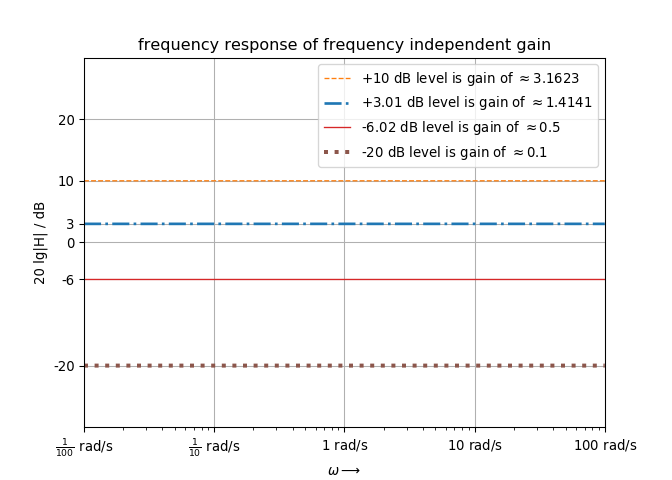
\includegraphics[width=0.5\textwidth]{fig_bode_mag_gain}
}
\subfloat[Zeros and poles in origin of $s$-plane, \eq{eq:Hs_sorted_for_Bode_dB_origin}.\label{fig_bode_mag_origin_zeros_poles}]{%
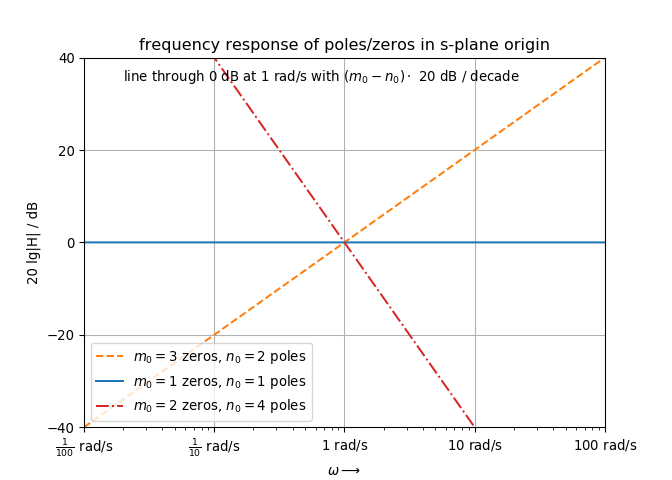
\includegraphics[width=0.5\textwidth]{fig_bode_mag_origin_zeros_poles}
}

\subfloat[Single, real zero, \eq{eq:Hs_sorted_for_Bode_dB_zero}.\label{fig_bode_mag_single_zero}]{%
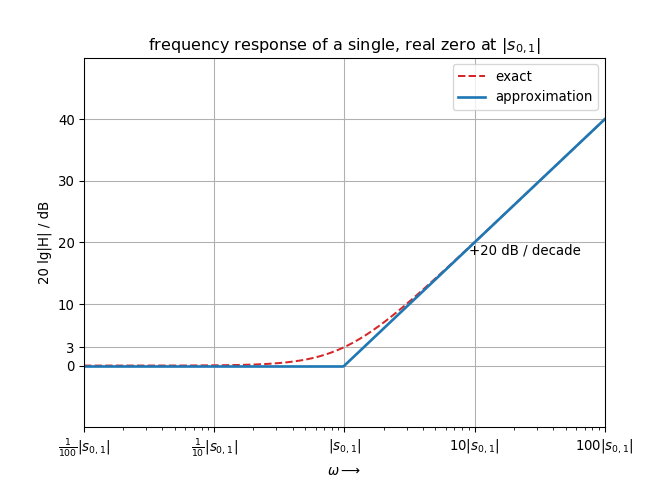
\includegraphics[width=0.5\textwidth]{fig_bode_mag_single_zero}
}
\subfloat[Complex conjugate pair of zeros, \eq{eq:Hs_sorted_for_Bode_dB_cczero}.\label{fig_bode_mag_conj_zeros}]{%
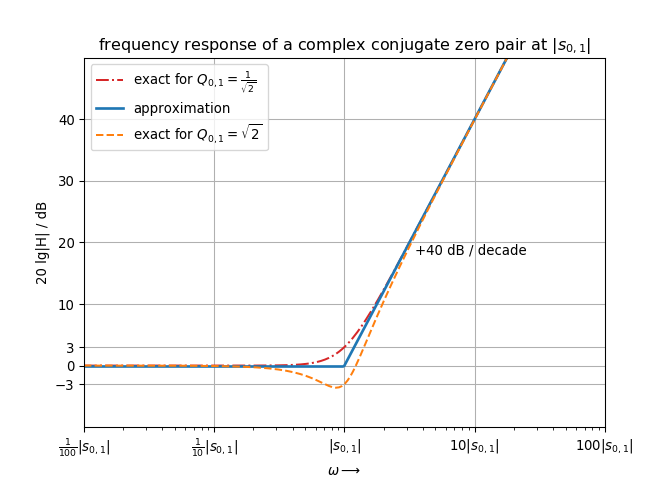
\includegraphics[width=0.5\textwidth]{fig_bode_mag_conj_zeros}
}

\subfloat[Single, real pole, \eq{eq:Hs_sorted_for_Bode_dB_pole}.\label{fig_bode_mag_single_pole}]{%
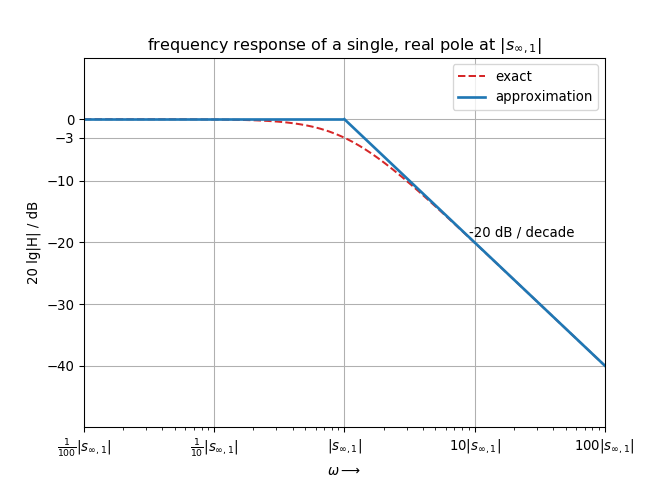
\includegraphics[width=0.5\textwidth]{fig_bode_mag_single_pole}
}
\subfloat[Complex conjugate pair of poles, \eq{eq:Hs_sorted_for_Bode_dB_ccpole}.\label{fig_bode_mag_conj_poles}]{%
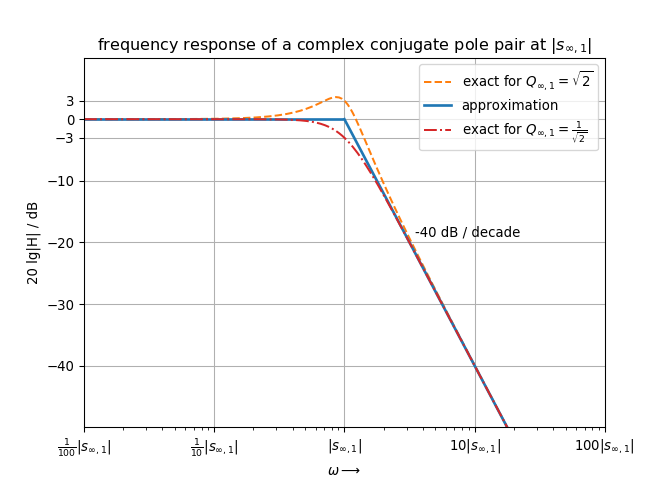
\includegraphics[width=0.5\textwidth]{fig_bode_mag_conj_poles}
}
\caption{Magnitude frequency response prototypes of zeros and poles for $s = \sigma + \im \omega$ with $\sigma=0$.}
\label{fig:magbodeprototype}
\end{figure}

Recall that for the Laplace variable $s=\sigma + \im\omega$ a chosen  $\sigma=0$ leads to the Fourier transform of $H(s)$, i.e. only harmonic oscillating events are considered.
This is precisely used to discuss the frequency response of an LTI system with
help of the Bode plot.
The magnitude Bode plot evaluates $20 \text{lg} |H(s)|\bigg|_{s=\im \omega}$.
The prototype systems \eq{eq:Hs_sorted_for_Bode_dB_gain} to \eq{eq:Hs_sorted_for_Bode_dB_ccpole} exhibit an interesting characteristic, when being plotted over a logarithmic frequency axis:
In the limiting cases, i.e. for frequencies much larger/smaller than around the pole/zero magnitude, the frequency response can be approximated by straight-line equations.
These approximations are visualised in Fig. \ref{fig:magbodeprototype}.

For example, for a single, real zero $s_{0,j}$ the prototype magnitude frequency response is $20 \text{lg}  \bigg|\frac{s}{s_{0,j}}-1\bigg|$
according to \eq{eq:Hs_sorted_for_Bode_dB_zero}.
For $|s| \ll |s_{0,j}|$, the value of one is dominating, yielding a line at 0 dB.
For $|s| \gg |s_{0,j}|$, the fraction is prevailing, yielding a line with a rise of 20 dB per decade (i.e. a tenfold increase of frequency).
The asymptotic characteristics changes exactly at $|s| = |s_{0,j}|$.
This is depicted in Fig. \ref{fig_bode_mag_single_zero}.

\section{Solution}
The Bode plot of \eq{eq:H_ODE} is depicted in Fig. \ref{fig:bode_ode}.

\begin{figure}[h!]
\centering
\subfloat[Magnitude, cf. Fig. \ref{fig_bode_mag_conj_poles}. Undamped natural frequency $\omega_0=\frac{5}{4}$ rad/s. $\omega_D=1$ rad/s, $Q_\infty=\frac{5}{6}$, $D=\frac{3}{5}$. Lowpass with slope of -40 dB/decade, i.e. -12 dB/octave (cf. $\omega=\frac{5}{2}$ rad/s and $\omega=5$ rad/s).
\label{fig_bode_mag_ode_example}]{%
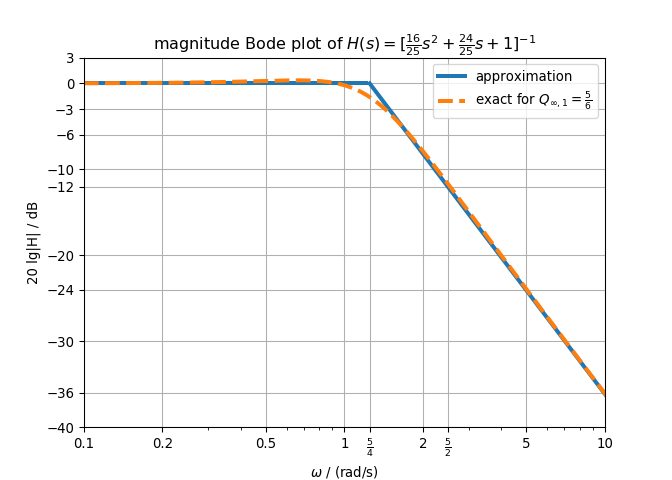
\includegraphics[width=0.6\textwidth]{fig_bode_mag_ode_example}
}

\subfloat[Phase. Note -90 deg at $\omega_0$, 0 deg for $\omega \rightarrow 0 $ and -180 deg for $\omega\rightarrow \infty$. \label{fig_bode_angle_ode_example}]{%
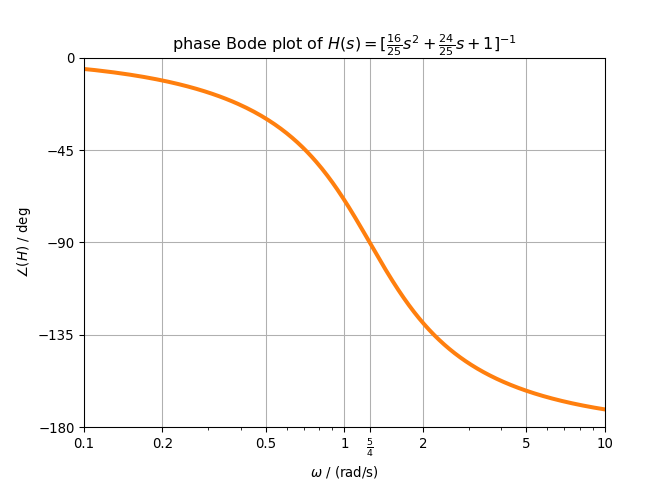
\includegraphics[width=0.6\textwidth]{fig_bode_angle_ode_example}
}
\caption{Bode plot of LTI system \eq{eq:H_ODE}.}
\label{fig:bode_ode}
\end{figure}

The Bode plot approximation with respect to magnitude is with above treatment as follows: The Laplace transform of \eq{eq:H_ODE} reads in general form
\begin{align}
H(s) = H_0 \frac{1}{(s-s_{\infty,1}) (s-s_{\infty,2})}
\end{align}
with $s_{\infty,1} = -\frac{3}{4}+\im$, $s_{\infty,2} = -\frac{3}{4}-\im$ and $H_0 = \frac{25}{16}$.
%
The poles constitute a complex conjugate pair, thus
$|s_{\infty,1}| = |s_{\infty,2}| = \frac{5}{4}$, $|s_{\infty,1}|^2 = |s_{\infty,2}|^2 = \frac{25}{16}$.
%
With \eq{eq:H0tilde}
\begin{align}
\tilde{H_0} = \frac{H_0}{|s_{\infty,1}|^2} = \frac{\nicefrac{25}{16}}{\nicefrac{25}{16}} = 1
\end{align}
and the suitable prototypes \eq{eq:Hs_sorted_for_Bode_dB_gain} and \eq{eq:Hs_sorted_for_Bode_dB_ccpole}
we get
\begin{align}
20 \text{lg} |H(s)| =
+20 \text{lg} |\tilde{H_0}|
-20 \text{lg} \bigg|\frac{s^2}{|s_{\infty,1}|^2} + \frac{s}{|s_{\infty,1}| Q_{\infty,1}} + 1\bigg|.
\end{align}
For
\begin{align}
\frac{s^2}{|s_{\infty,1}|^2} + \frac{s}{|s_{\infty,1}| Q_{\infty,1}} + 1
\end{align}
we find that $Q_{\infty,1}=\frac{5}{6}$, and since $20 \text{lg} |\tilde{H_0}|=0\mathrm{dB}$, we have just to deal with
\begin{align}
20 \text{lg} |H(s)| =
-20 \text{lg} \bigg|\frac{s^2}{|s_{\infty,1}|^2} + \frac{s}{|s_{\infty,1}| Q_{\infty,1}} + 1\bigg|.
\end{align}
This directly corresponds to the prototype \eq{eq:Hs_sorted_for_Bode_dB_ccpole}, which
is schematically depicted in Fig. \ref{fig_bode_mag_conj_poles}.
%
In Fig. \ref{fig_bode_mag_ode_example} the approximation is plotted as blue graph with a slope of -40 dB per decade starting at $\omega_0 = |s_{\infty,1}|=\frac{5}{4}$.
The slope is also often referenced to frequency doubling, i.e. here -12 dB/octave\footnote{Slopes correspond to the order $o$ of a lowpass system, hence $-o\cdot 20$ dB/decade, $-o\cdot 6$ dB/octave. We deal with $o=2$ order system due to two poles.}, cf. this at frequencies $\omega=2.5, 5, 10$ rad/s in the plot.

The exact solution with $Q_{\infty,1}=\frac{5}{6}$ and thus exact magnitude plot is depicted as orange graph. This pole quality leads to $\approx 0$ dB at $\omega_D=1$ rad/s and a very flat response for frequencies up to $\omega_D$
with only very slight overshoot at around $\omega = 0.5$ to $0.8$ rad/s.
Note that by decreasing $Q\rightarrow 0.5$ (thus $D\rightarrow 1$) the system becomes higher damped. A special case --- called Butterworth filter characteristic --- is
$Q = \frac{1}{\sqrt{2}}$, where -3.01 dB at $\omega_0 = \frac{5}{4}$ rad/s is obtained, cf. Fig. \ref{fig_bode_mag_conj_poles}.
By increasing $Q$ (thus $D\rightarrow 0$) less damping is achieved, resulting in a more resonant system characteristic at $\omega_0$.
%
The phase response of the 2nd order lowpass under discussion is depicted
in Fig. \ref{fig_bode_angle_ode_example}.
It exhibits typical phase shift of zero at very low frequencies near 0 rad/s and -180 deg phase at very high frequencies.
A phase shift of -90 deg is generally obtained at $\omega_0$ independently of
the pole quality.
This is the reason $w_0$ is often referred to as the cut frequency
of the lowpass filter, since it marks the borderline between the two general characteristics: $\omega \ll \omega_0$ defines the so called passband, $\omega \gg \omega_0$ defines the so called stop band of the lowpass. The transition
(the steepness of the slope and its style) between the two bands is
determined by the filter order (number of poles) and characteristics (position of poles within $s$-plane).
For details there are numerous book on filter design. The standard reference Tietze, U.; Schenk, Ch.; Gamm, E. (2008): "\textit{Electronic Circuits --- Handbook for Design and Applications}", Springer, 2nd ed. is a good starting point for filter design.





\section{Additional Task/Example: Bandpass 2nd order}

If we put a zero in origin $s_0=0$, a pole at $s_{\infty,1}=-0.1$ and one
pole at $s_{\infty,2}=-10$ we obtain a 2nd order bandpass system.
With a gain factor $H_0$ = 10 to yield 0 dB in the passband
the Laplace transfer function reads
\begin{align}
H(s) = H_0\frac{s-s_{0,1}}{(s-s_{\infty,1})(s-s_{\infty,2})} = 10\frac{(s-0)}{(s-(-0.1))(s-(-10))}
=\frac{100 s}{10 s^2 + 101 s + 10}.
\end{align}
%
We might elaborate the magnitude frequency response prototypes for this
LTI system to obtain a Bode plot approximation.
%
Four contributions from \eq{eq:Hs_sorted_for_Bode_dB_gain} to \eq{eq:Hs_sorted_for_Bode_dB_ccpole} need to be considered
\begin{align}
20\mathrm{lg}|H(s)| = 20\mathrm{lg}|\tilde{H_0}| + 20\mathrm{lg}|s| - 20\mathrm{lg}|\frac{s}{|s_{\infty,1}|}-1|
- 20\mathrm{lg}|\frac{s}{|s_{\infty,2}|}-1|,
\end{align}
and \eq{eq:H0tilde} becomes
\begin{align}
\tilde{H_0} = \frac{H_0}{|s_{\infty,1}| \cdot |s_{\infty,2}|} = 10 \rightarrow 20\mathrm{lg}|\tilde{H_0}| = 20 \mathrm{dB}.
\end{align}
In Fig. \ref{fig:fig_bode_mag_bandpass_example} the prototypes, that needs to be additively superimposed are depicted as blue, orange, green and red graphs.
The resulting approximation of the 2nd order bandpass is shown in black, the exact magnitude frequency response is shown as thin, grey curve.
\begin{figure}[h!]
\centering
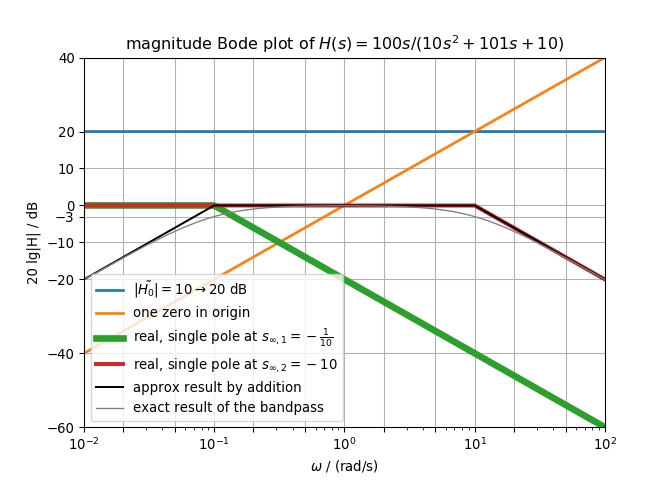
\includegraphics[width=0.75\textwidth]{fig_bode_mag_bandpass_example}
\caption{Magnitude Bode plot of 2nd order Bandpass.}
\label{fig:fig_bode_mag_bandpass_example}
\end{figure}



\bibliographystyle{IEEEtranSA.bst}
\bibliography{literature}
\end{document}
